\documentclass{article}
\usepackage[utf8]{inputenc}
\usepackage{multirow}
\usepackage{multicol}
\usepackage{pdfpages}

\title{NAC-EWASS 2020}

\begin{document}

\maketitle

\section{The NAC in 2020}
As EWASS will be coming to Leiden in 2020, a proposal will be drafted to organize the NAC as part of EWASS. This will give young researchers such as PhDs an opportunity to simulateously attend this large astronomical conference. It will also avoid the two conferences being be back to back in a short time frame. It is important to keep our Dutch identity within such a large gathering of astronomers. This document outlines ideas and plans on how we think we can achieve this. We will aim for an eco-friendly gather: no plastic bottles and vegetarian food.

\subsection{Comittees}
\begin{center}
    \begin{tabular}{ccc}
        \textbf{NAC SOC }& \textbf{NAC LOC} & \textbf{NAC+EWASS LOC} \\
        \hline
        Simon Portegies Zwart & Simon Portegies Zwart & Dirk van Dam \\
        Jan Lub               & Martijn Oei           & Rafa\"el Mostert \\
                              & Frits Sweijen         & Martijn Oei \\
                              & Martijn Wilhelm       & Lydia Stofanova
    \end{tabular}
\end{center}
\subsection{Venue}
The venue is the Holiday Inn. Multiple small to medium rooms are available and one large main hall, for (probably) the plenary sessions of EWASS. There is a vide available, which we may be able to claim as the ``Dutch Garden'' with an activity such as a Lego sculpture to build, a puzzle make or something else to keep people entertained outside the talks, focussing on a Dutch theme within astronomy.

In total there are 12 meeting rooms and one large hall, the convention center. The following pages show the rooms with their capacities in various setups and the layout of all the rooms at a 1 to 250 scale, respectively.

\subsubsection*{Meeting rooms}
On request, Holiday Inn can provide extension cords for the meeting rooms. They can prepare the rooms in a requested setup (chairs/tables) once per day.

\subsubsection*{Convention Center}
The convention center and its vide do not have airconditioning and will get hot if we get warm weather. We should think about ways to cool or ventilate the room. Holiday Inn does not provide this, so we should bring fans (for example) ourselves.

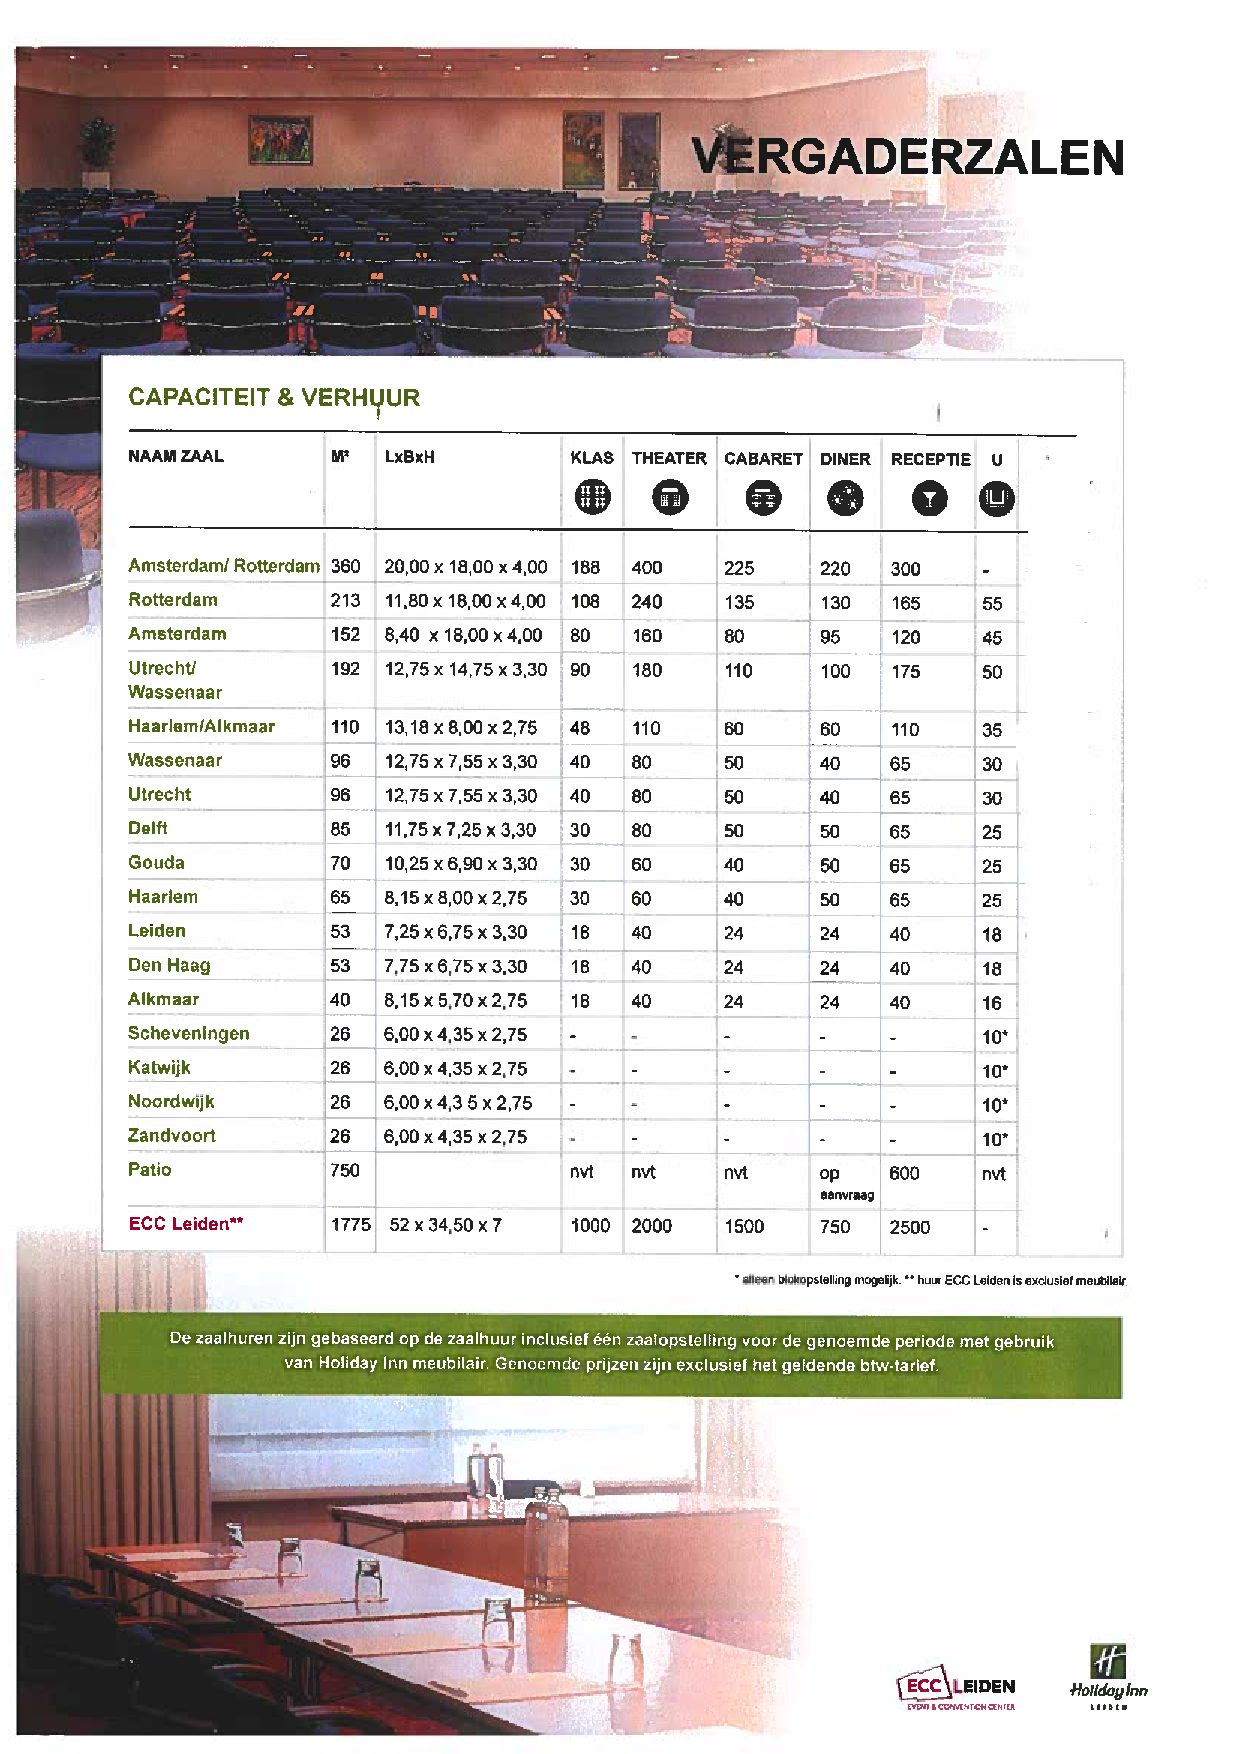
\includepdf{zalen_capaciteit.pdf}
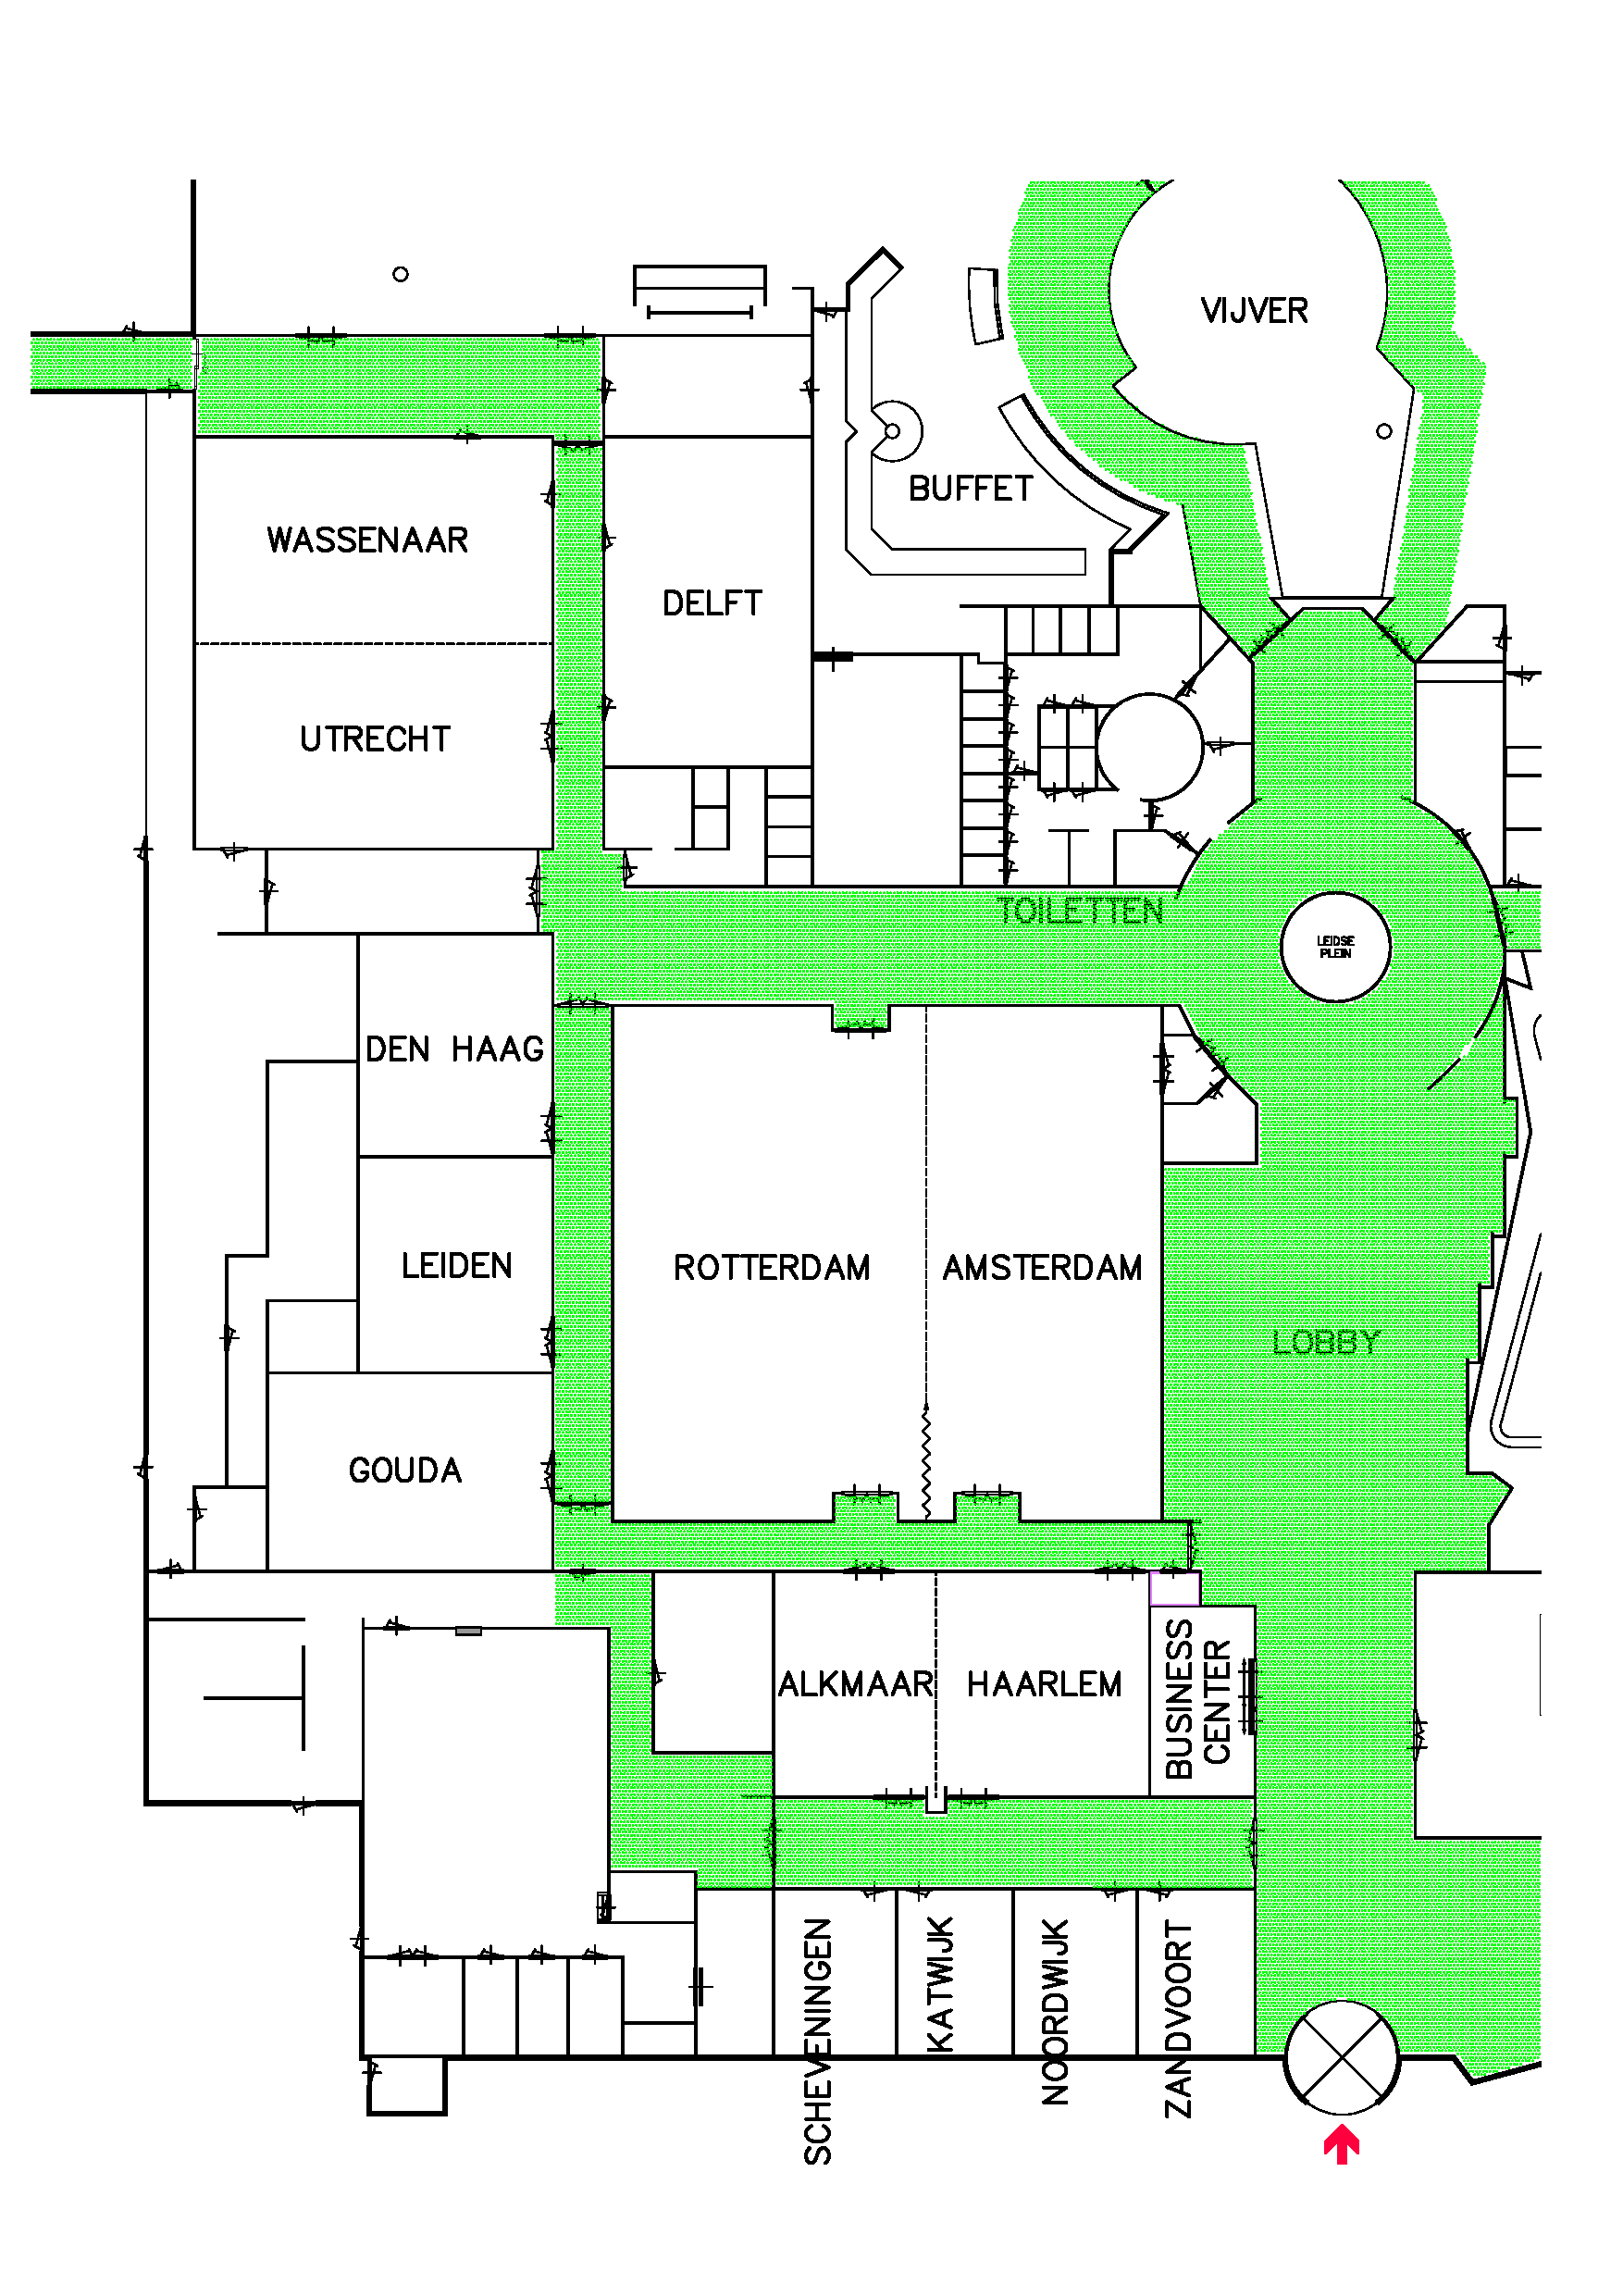
\includepdf{zalen_vloerplan_1_op_250.pdf}

\subsection{Posters}
EWASS will not use physical posters, but present them on interactive screens instead. For the NAC we will stick to physical paper posters. These can be put up, for example, in the long hallway leading to the large room, guiding everyone to walk past them.

\subsection{Dinner}
A Dutch NAC dinner separate from the EWASS dinner, which should be included in the conference fee.

\section{NAC 2020 Program}
We aim for four half days of NAC during the EWASS conference. These will run from 13:00 to 17:00 each day. A range of topics will need to be covered by both talks and ``hack'' sessions. This will require two rooms for each half day; one for each.

\begin{tabular}{ll|l}
    & \multicolumn{2}{c}{\textbf{DAY STARTS}} \\
    \cline{2-3}
    \textbf{13:00 - 13:30} & \multicolumn{2}{c}{Vici talk} \\
    %\cline{2-3}
    \textbf{13:30 - 15:00} & PhD/PostDoc talks, topic 1 & Hack session topic 2 \\
    %\cline{2-3}
    \textbf{15:00 - 15:30} & \multicolumn{2}{c}{Coffee break} \\
    %\cline{2-3}
    \textbf{15:30 - 16:30} & PhD/PostDoc talks, topic 3 & Hack session topic 4 \\
    %\cline{2-3}
    \textbf{16:30 - 17:00} & \multicolumn{2}{c}{Spinoza talk} \\
    \cline{2-3}
    & \multicolumn{2}{c}{\textbf{DAY ENDS}}
\end{tabular}\\%

\subsection{Talks}
Each day will start with a focussed ``tough talk'', given by an invited speaker who has won a Vici grant. Afterwards, there will be 2 hours and 30 minutes available for student talks, of 20 minutes each (this leaves 10 minutes of room for switching speakers, technical difficulties etc.). The day is closed by another invited talk, this time by someone who has won a Spinoza laureat to give a lighter talk, giving a broader overview of the science in that field.

The talks will cover a wide range of topics. Each session before and after the coffee break will have its focus on one. Below is a proposed list of topics:
\begin{multicols}{2}
    \begin{enumerate}
        \item Outreach
        \item Instrumentation
        \item Simulations and modeling
        \item Multi-messenger astronomy
        \item Imaging
        \item Spectroscopy
        \item Theory
        \item Inteferometry
    \end{enumerate}
\end{multicols}

\subsection{Hack sessions}
During the talks, there will be more hands-on ``hack'' sessions in parallel. Here people can come together to, for example, go to a tutorial, a lecture or in another way more interactive session to learn about particular topics, such as outreach or data reduction. A list of ideas for these topics is summarized below. Some of these session could be more hands-on, with participants actually doing work, while others that are more or too involved to do no the spot (e.g. LOFAR, GAIA), could perhaps be more like a talk/discussion session to give more insight in e.g. how to obtain and reduce the data.

\begin{multicols}{2}
    \begin{enumerate}
        \item Training on outreach
        \item AMUSE data reduction
        \item Python in astronomy
        \item Machine learning
        \item LOFAR data reduction
        \item NOVA-6
        \item COSMOSIM
        \item GAIA
    \end{enumerate}
\end{multicols}

\section{Speakers}
Each session will need at least two invited speakers: one Vici grant and one Spinoza laureat. This section will list possible speakers, to invite, sorted by applicable topics. Institutes to consider are:

\begin{multicols}{2}
    \begin{enumerate}
        \item University of Groningen (RuG)
        \item Leiden University (LU)
        \item Radbout University (RU)
        \item VU Amsterdam (VU)
        \item ASTRON
        \item SRON
        \item NIKHEF
        \item Belgians
    \end{enumerate}
\end{multicols}

\subsection{Outreach}
\begin{enumerate}
    \item Pedro Russo (LU)
    \item Peter Barthel (RuG)
    \item Joeri van Leeuwen (UvA, Vici)
    \item Bas Haring
    \item Ionica Smeets
\end{enumerate}

\subsection{Instrumentation}
\begin{enumerate}
    \item Paul Groot (RU)
    \item Peter Jonker (RU)
    \item Jelle Kaastra (SRON)
    \item Hiroki Akamatsu (SRON)
\end{enumerate}

\subsection{Simulations and modeling}
\begin{enumerate}
    \item Adrian Hamers
    \item Amina Helmi (RuG, Vici + Spinoza)
\end{enumerate}

\subsection{Multi-messenger Astronomy}
\begin{enumerate}
    \item Gijs Nelemans (RU, Vici)
    \item Michiel van der Klis (UvA, Spinoza)
    \item Heino Falcke (RU, Spinoza)
\end{enumerate}

\subsection{Imaging}
\begin{enumerate}
    \item Marc Verheijen (RuG, Vici)
    \item Ewine van Dishoeck (LU, Spinoza)
\end{enumerate}

\subsection{Spectroscopy}
\begin{enumerate}
    \item Ignas Snellen (LU, Vici)
    \item Xander Tielens (LU, Spinoza)
\end{enumerate}

\subsection{Theory}
\begin{enumerate}
    \item Sera Markoff (UvA, Vici)
    \item Erik Verlinde (UvA)
    \item Chris van den Broek (NIKHEF, Vici)
\end{enumerate}

\subsection{Interferometry}
\begin{enumerate}
    \item Heino Falkce (RU, Spinoza)
\end{enumerate}

\subsection{Newly hired researchers}
\begin{enumerate}
    \item Aurora Simionescu (LU)
    \item Yamilia Miguel (LU)
    \item Elisa Constantini (UvA)
    \item Elena Sellentin (LU)
\end{enumerate}
\end{document}
